\chapter{Results}


\section{Loading times}
\label{Loading times}
Table \ref{tbl:loadingtimes} shows an overview of the initial full page loading
times for the legacy TS (version 2.1.0) and the new TS (version 3.4.0). That is,
a page load from a new browser tab with all caches removed.

This test is performed with the timeline panel of Google Chrome 50.0.2661.86 (64-bit).

\begin{table}
  \begin{center}
    \begin{tabular}{| l | l | l | l | l |}
    \hline
     & TS 2.1.0 (Dojo) & TS 3.4.0 (Dojo + Polymer) & difference & difference (\%) \\ \hline
    \textbf{Loading} & 44.5ms & 112.4ms & +67.9ms & +152.58\%  \\ \hline
    \textbf{Scripting} & 1227.6ms & 1187.6ms & -40ms & -3,26\% \\ \hline
    \textbf{Rendering} & 29.7ms & 171.0ms & +141.3ms & +475,76\% \\ \hline
    \textbf{Painting} & 7.5ms & 36.1ms & +28.6ms & +381.33\% \\ \hline
    \textbf{Other} & 106.4ms & 335.9ms & +229.5ms & +215,69\% \\ \hline
    \textbf{Idle} & 213.6ms & 775.1ms & +561.5ms & +262,87\% \\ \hline \hline
    \textbf{Total} & \textbf{1.63s} & \textbf{2.62s} & \textbf{+990ms} & \textbf{+60,73\%} \\ \hline
    \end{tabular}
  \end{center}
  \caption{Page loading times for TS 2.x and 3.x}
  \label{tbl:loadingtimes}
\end{table}

It is expected that the TS 3.x has higher values for everything in this table,
because it loads two front-end libraries (Dojo \& Polymer).

Notable is the decrease of scripting time for the TS 3.x relative to the
TS 2.x. This is because Dojo is minified and packaged into one JavaScript file
in the TS 3.x release, where as in the TS 2.x release it was not.
Also, because this test is performed in Google Chrome, which has native support
for Web Components, very little scripting needs to be done.
This result will be different in other browsers like Mozilla Firefox, where
Web Components support needs to be emulated. Then again, the lazy loading system
largely removes this overhead from the initial page loading time, so only minor
differences would be expected here.

Rendering time has increased the most going from TS 2.x to TS 3.x. This makes
sense as Polymer renders everything on the front-end, whereas Dojo used to render
everything server-side.
During initial page load this rendering load is primarily caused by the rendering
of the left side menu.
The increase of painting time follows the same logic as the rendering time.

Also notable is the increase of idle time. This means that the browser needs to
wait for a task to finish before it can start another.
This is caused because the TS 3.x loads the default panel after the initial page
load. Which means the TS makes extra network request, to fetch an interface panel,
right after initializing. This is counted with the initial page load.
TS 2.x just shows a blank page, it loads no default panel.
Because the browser needs to wait for the extra network requests to finish before
it can render the default panel, the idle time goes up by a lot.

In total, the initial page loading time increased with about 60\%, which is an
acceptable increase given the new TS runs 2 libraries concurrently.

\section{CPU consumption}
Both TS releases have negligible CPU usage when doing a fresh page load, and
stay at 0\% CPU usage when the user is not interacting with the system.

TS 3.x uses hardware acceleration for it's animations since they are all made
using CSS transform properties or using Web Animations\cite{webanimations}.
The only exception to this is the `paper-spinner` element. Which displays a
loading animation.
The TS 2.x release did not have any animations.

% \begin{figure}[H]
%   \centering
%   
\includegraphics[width=.1\textwidth]{images/paper-spinner}
%   \caption{The most CPU intensive component of the TS 3.x interface}
%   \label{fig:paper-spinnger}
% \end{figure}

\section{Memory consumption}
Chapter \ref{Memory leaks in Dojo} described the memory leak problems in TS 2.x.
It showed a clear memory leak problem that needs addressing in TS 3.x.

Image \ref{fig:ts3_memory} showed that the new interface contains no memory leaks,
unless of course a panel developer creates one. This is why the `ts-ajax` and
`auto-update` elements in the `common-elements` package have been equipped with
ways to detect a circular reference, as they are the most likely to be used in one.

Unfortunately it also showed in figure \ref{fig:ts3_legacy_memory} that legacy
panels in the new TS still suffer from this memory leak. This is because the
circular references causing the memory leak reside in the Dojo library itself,
and thus would be impractical to address.
Therefore, any interface that included auto-refreshes had the highest priority
to be converted to a new TS 3.x interface.

Because TS 3.x uses client-side interface rendering rather than server-side as
the TS 2.x did, it uses more memory from the browser.

Chapter \ref{Loading times} already described that in TS 3.x the memory used
by an interface panel will be released after it switches to another panel.
It also described that in TS 2.x the memory consumption grows linearly with the
amount of panels loaded by the user.

To test the difference in memory consumption, both TS versions were opened in
a new tab while memory consumption is monitored. No panels are loaded, the
interfaces are just left for 120s. The mean memory consumption in those 120s is
then taken as the mean memory consumption for that TS release.
The results of this test are shown in table \ref{tbl:memoryusage}.

\begin{table}
  \begin{center}
    \begin{tabular}{| l | l | l |}
    \hline
     & Google Chrome & Firefox \\ \hline
    \textbf{TS 2.1.0 (Dojo)} & 20.051MB & 7.06MB \\ \hline
    \textbf{TS 3.4.0 (Dojo + Polymer)} & 24.564MB & 10.96MB \\ \hline
    \textbf{difference} & +4.513MB & +3.9MB \\ \hline
    \textbf{difference (\%)} & \textbf{+22.51\%} & \textbf{+55.24\%} \\ \hline
    \end{tabular}
  \end{center}
  \caption{Memory usage for TS 2.x and 3.x in Mozilla Firefox and Google Chrome}
  \label{tbl:memoryusage}
\end{table}

\section{Functionality}
TS 3.x has functionally more capabilities for the interface than TS 2.x had.
More importantly, the TS interface is now no longer bound to one framework.
Any Web Component can be used, and extra functionality can be developed in-house.
This unlike TS 2.x where developers were functionally bound to the elements the Dojo
developers provided.

This makes TS 3.x far more easy to change, and thus more ready for the future.

\section{SDK improvements}
The fact that multiple programming languages are no longer placed into one file,
but distributed across multiple files, makes the developing an interface panel
a lot easier.

The Web Components approach to build interfaces gives developers a set of
powerful tools that are easy to use and extend.
% \subsection{Decreased development time}

% \section{Documentation}

\section{Developed panels}
The Control Panels are a set of custom interfaces, developed for an individual cell.
The other panels however occur on every cell. And are upgraded as part of the
new TS release.
\subsection{Commands}
The new commands panel use the `command-input` element for its input. Making it
easily extendible to understand more input types (e.g. vectors).
Currently it understands number, int, long, unsigned int, unsigned long, short,
unsigned short, string, double, and float input.
\begin{figure}[H]
  \centering
  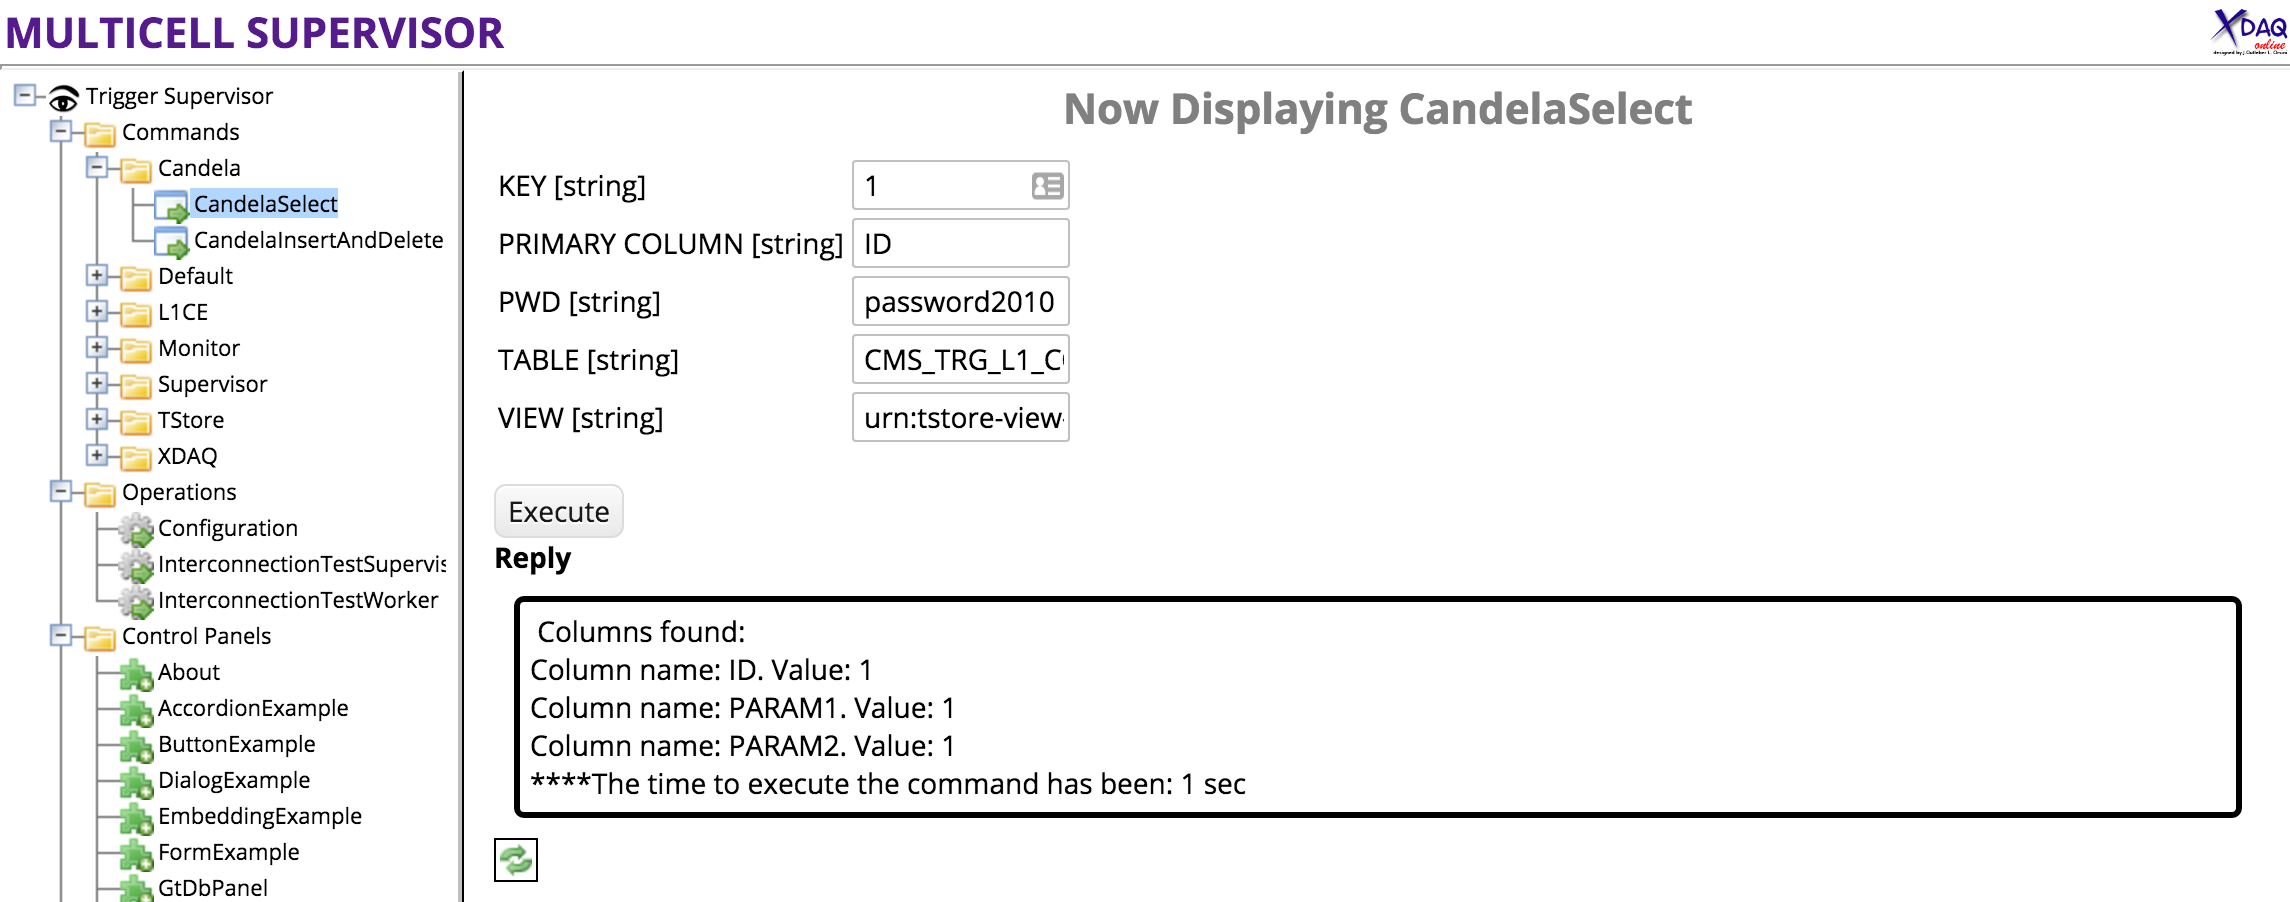
\includegraphics[width=\textwidth]{images/ts2_commands}
  \caption{TS 2.x commands panel}
  \label{fig:ts2_commands}
  \centering
  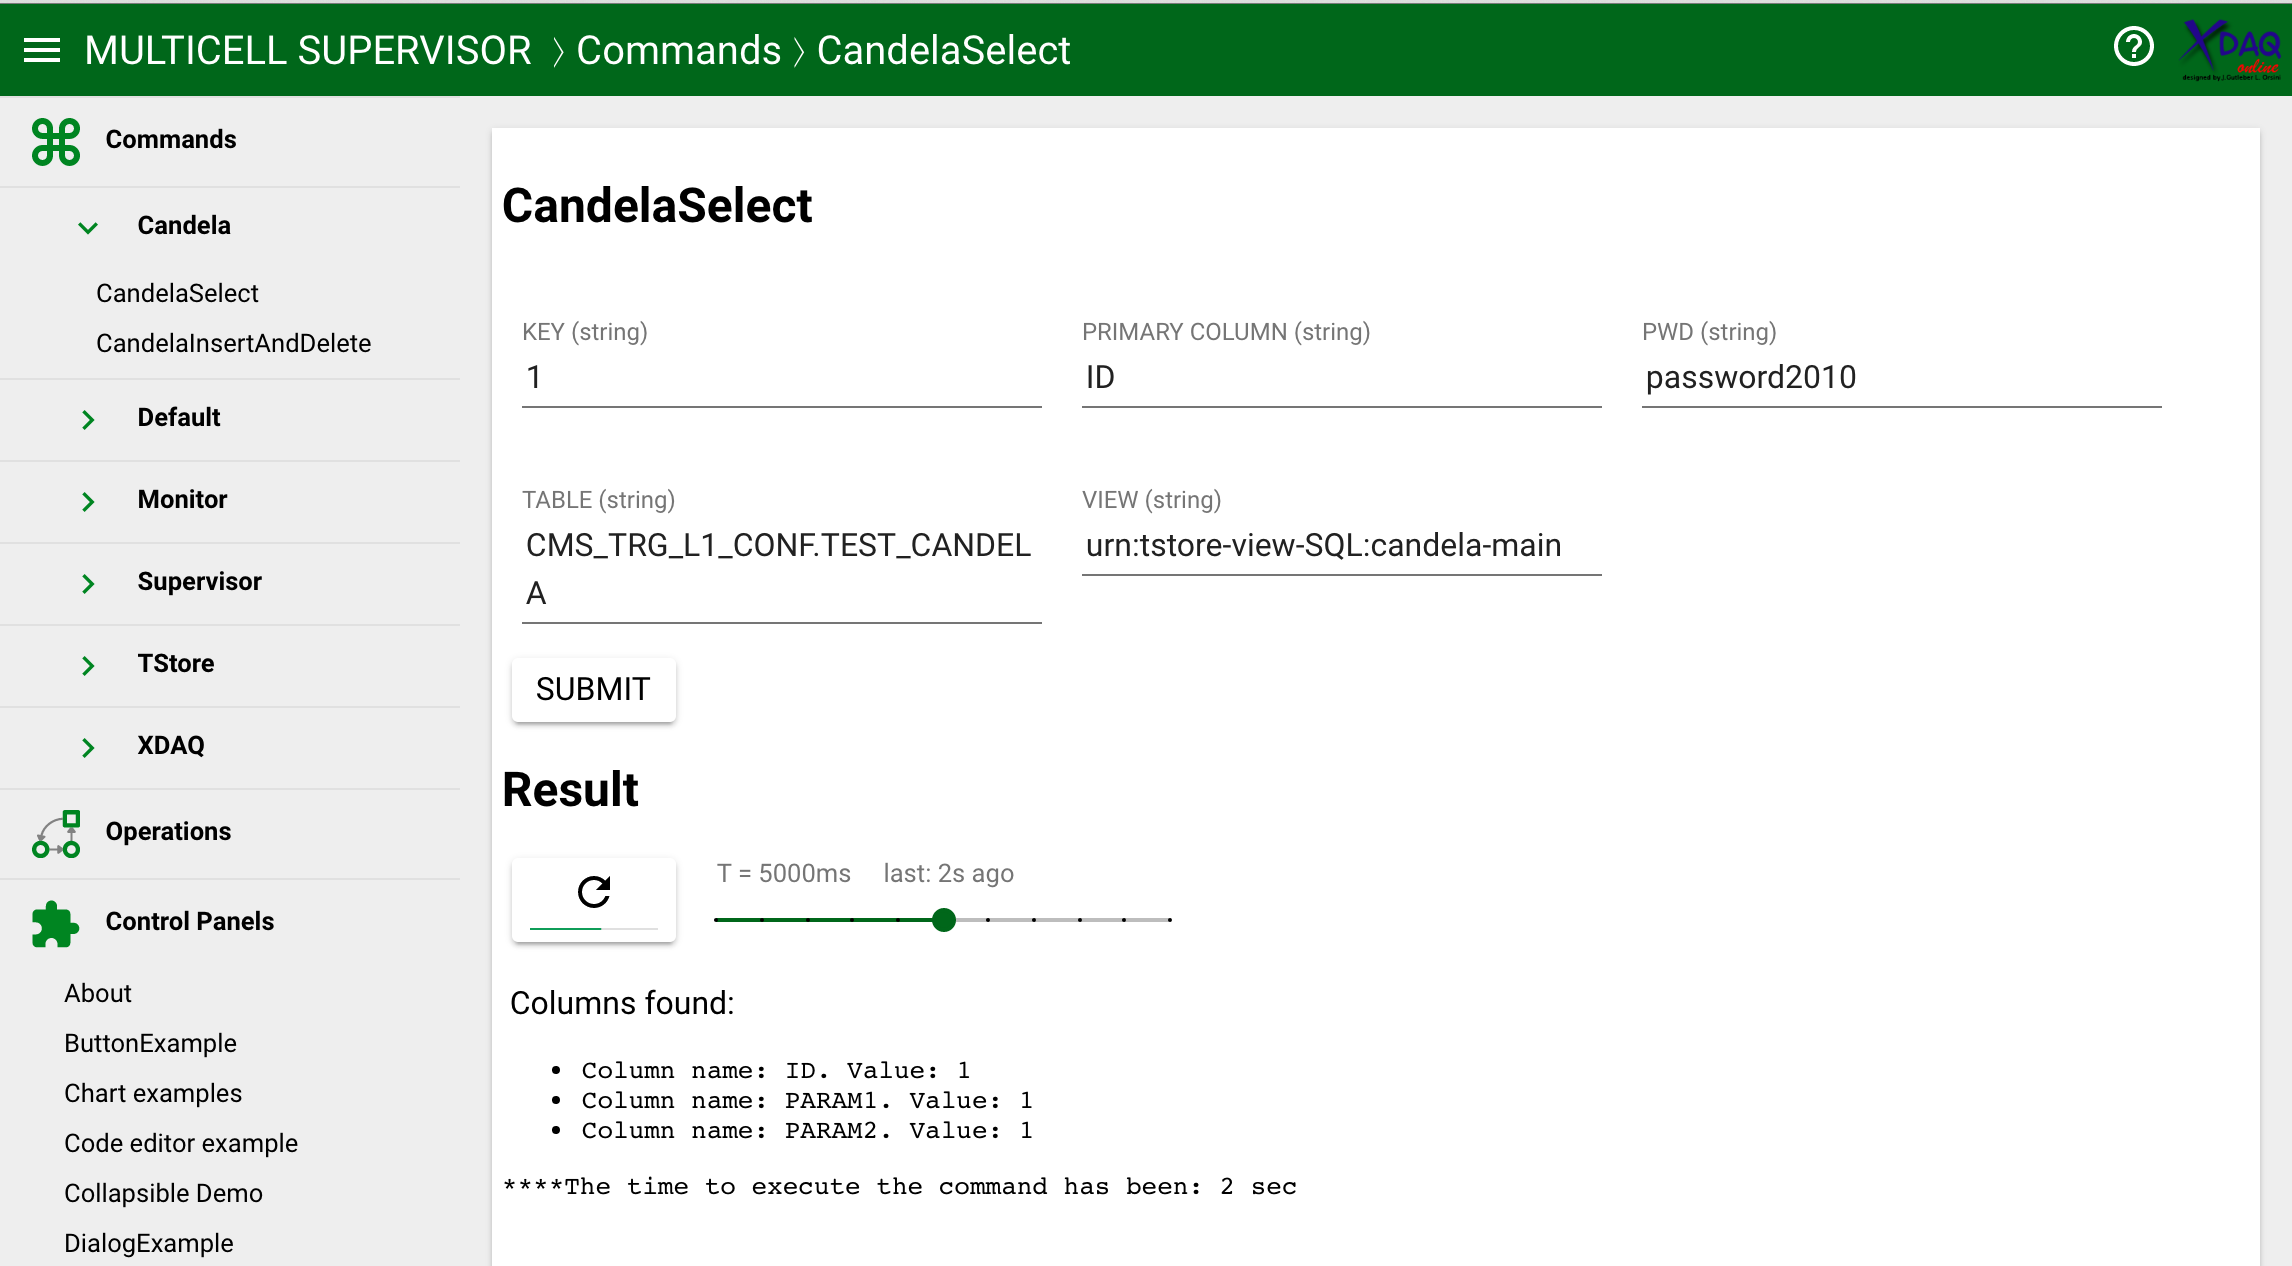
\includegraphics[width=\textwidth]{images/ts3_commands}
  \caption{TS 3.x commands panel}
  \label{fig:ts3_commands}
\end{figure}

\subsection{Operations}
The TS 2.x operations panel had some problems with auto-updating.
The state diagram tended to update very late, if it updated at all.
Result data and new available commands usually took more than 10 seconds to
show up in the interface.

The new operations panel is now far more responsive.
The state diagram is available when clicking on an icon, as it was deemed a
waste of space to show it by default.
\begin{figure}[H]
  \centering
  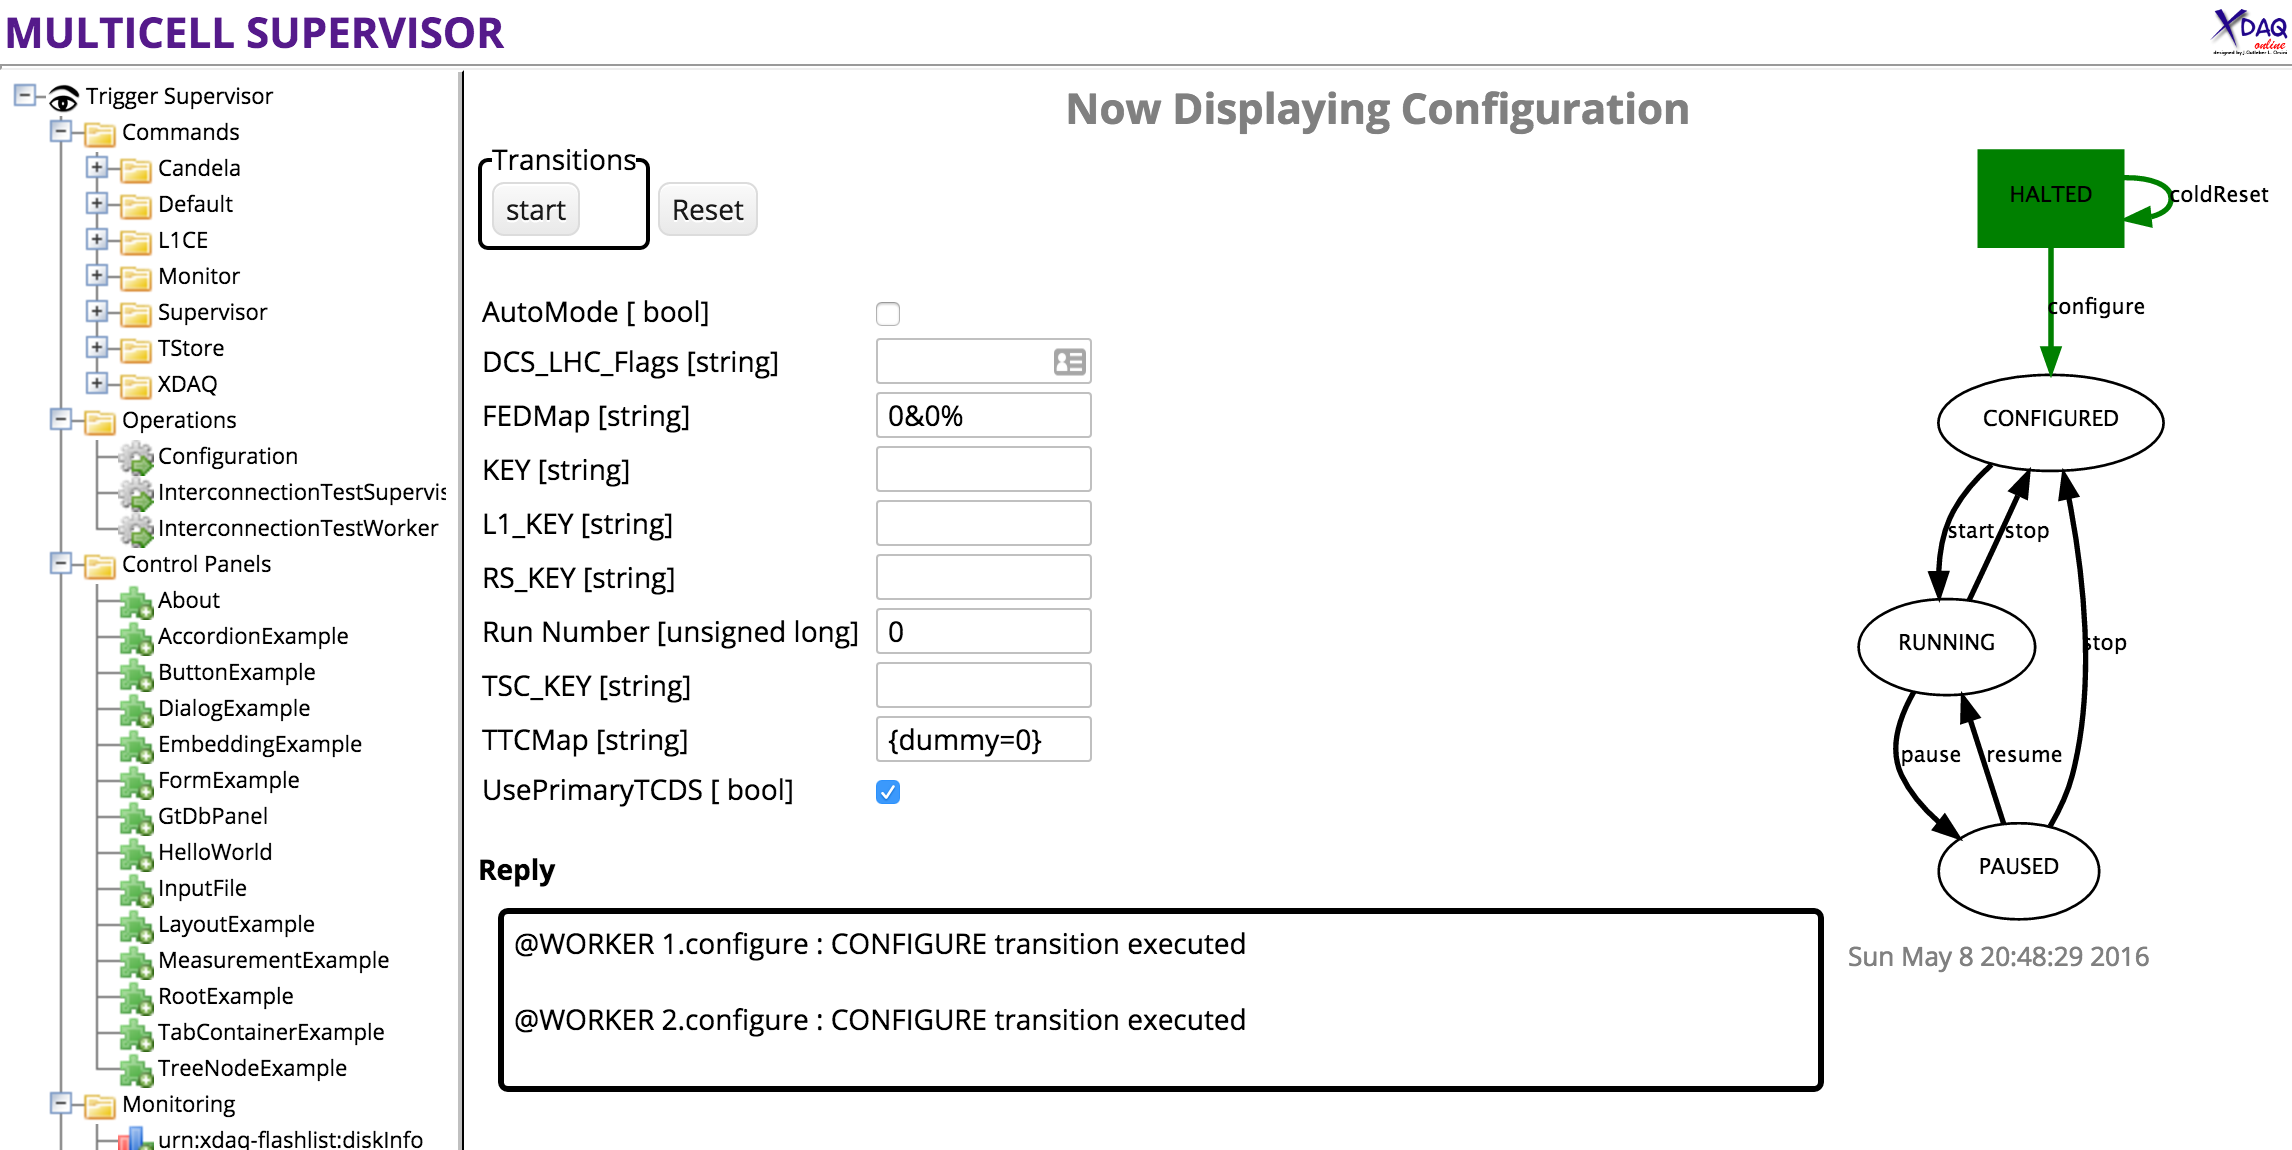
\includegraphics[width=\textwidth]{images/ts2_operations}
  \caption{TS 2.x operations panel}
  \label{fig:ts2_operations}
  \centering
  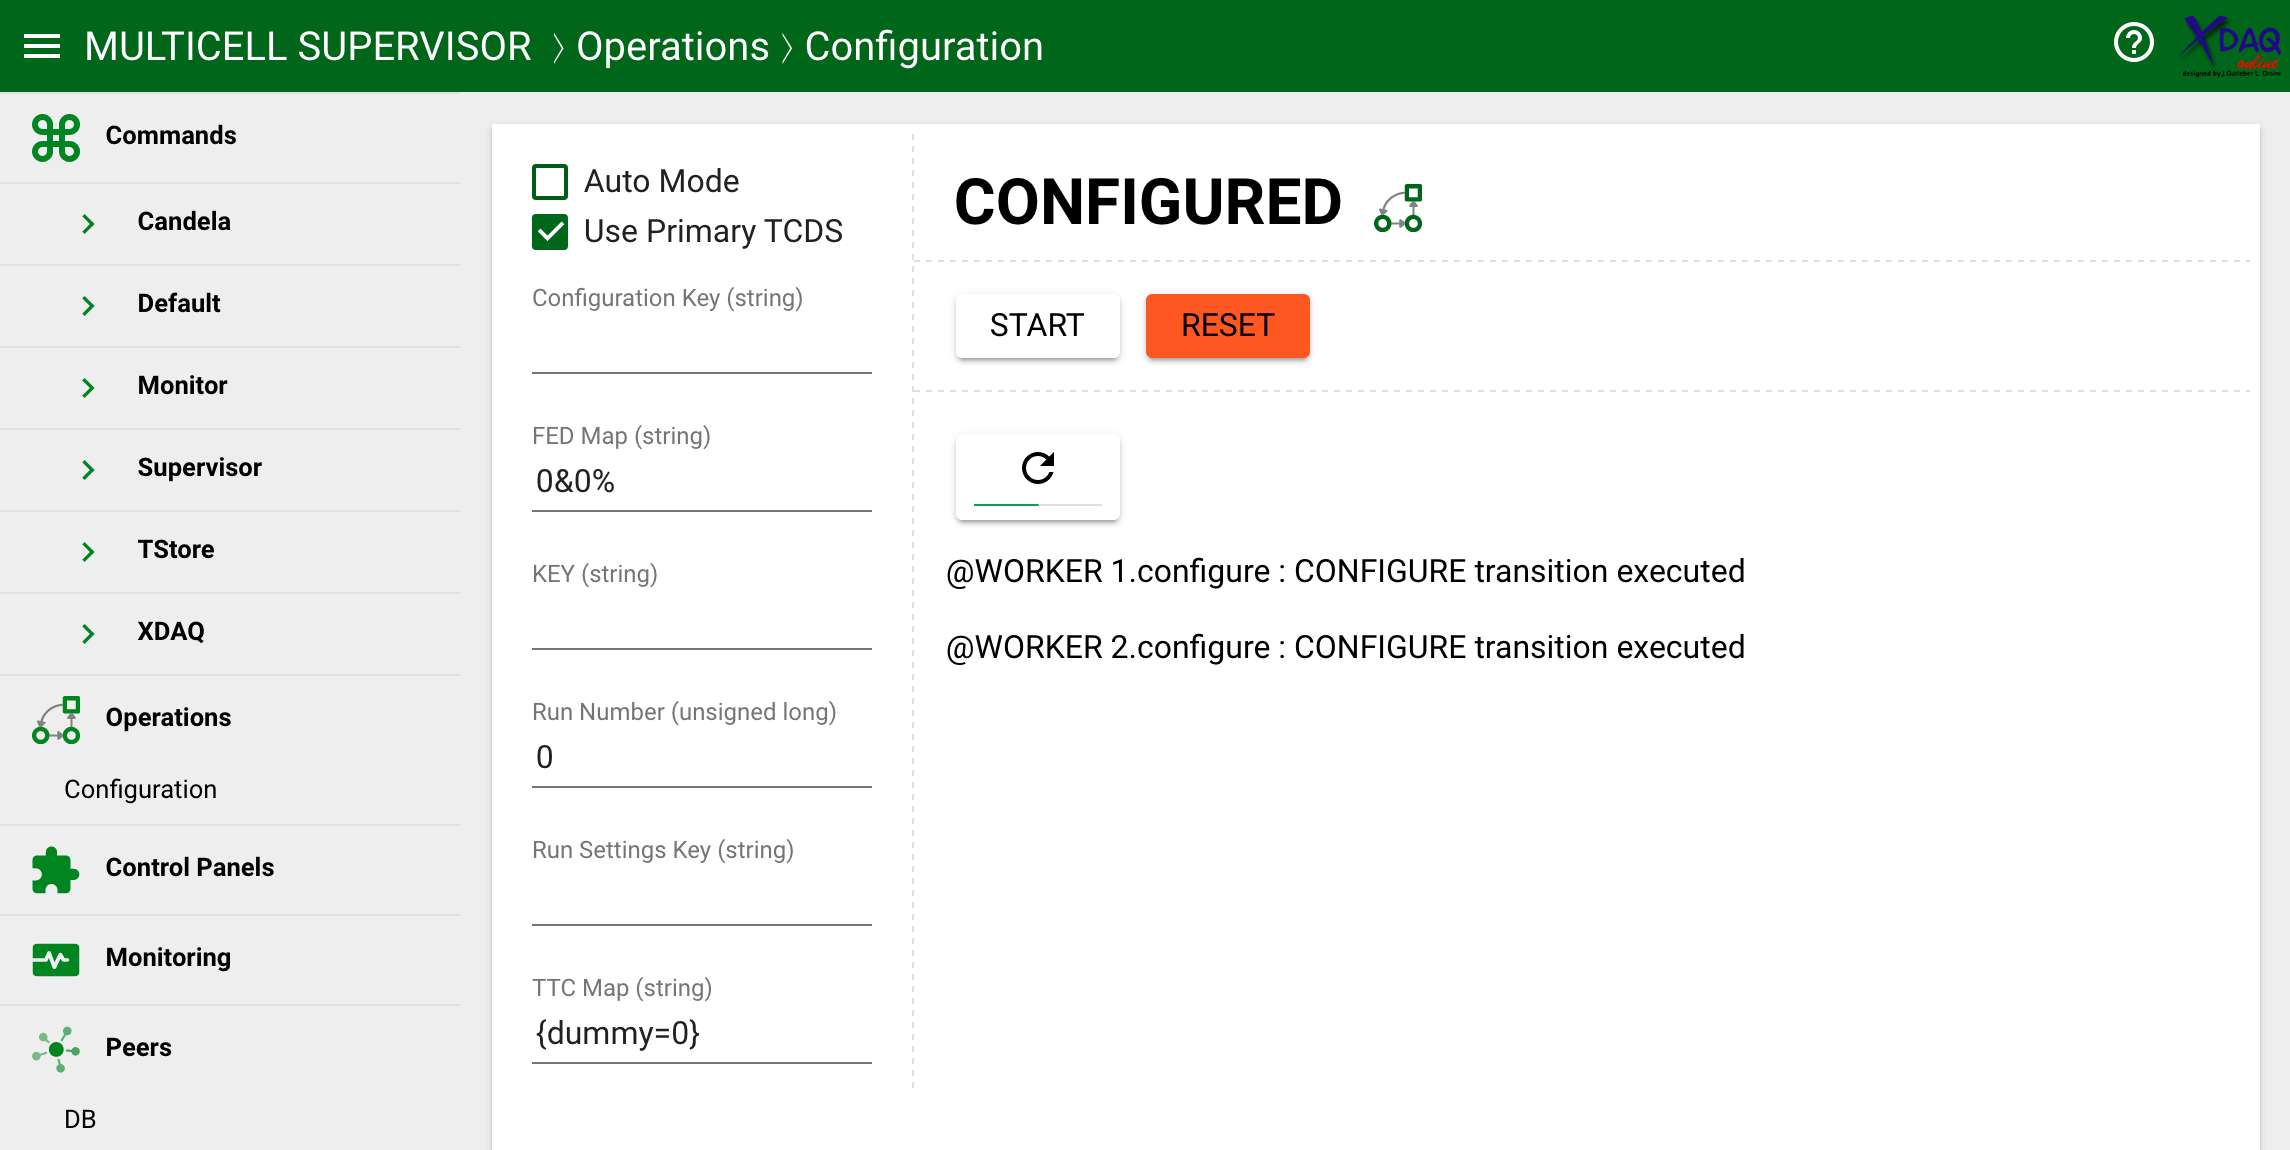
\includegraphics[width=\textwidth]{images/ts3_operations}
  \caption{TS 3.x operations panel}
  \label{fig:ts3_operations}
\end{figure}

\subsection{Flashlists}
% TODO definition of a flashlist
A flashlist is a more abstract interface designed to display tabular data.
This data can change with a regular interval. A table cell can contain a string,
date, number, or another table.

The flashlist panels now have a user-configurable auto-update function.
The flashlist can deploy custom renderers in the table depending on the data type,
for example a date will be shown as relative time (e.g. 9 minutes ago), instead
of just showing a time stamp. This list of custom renderers can be extended
easily.

\begin{figure}[H]
  \centering
  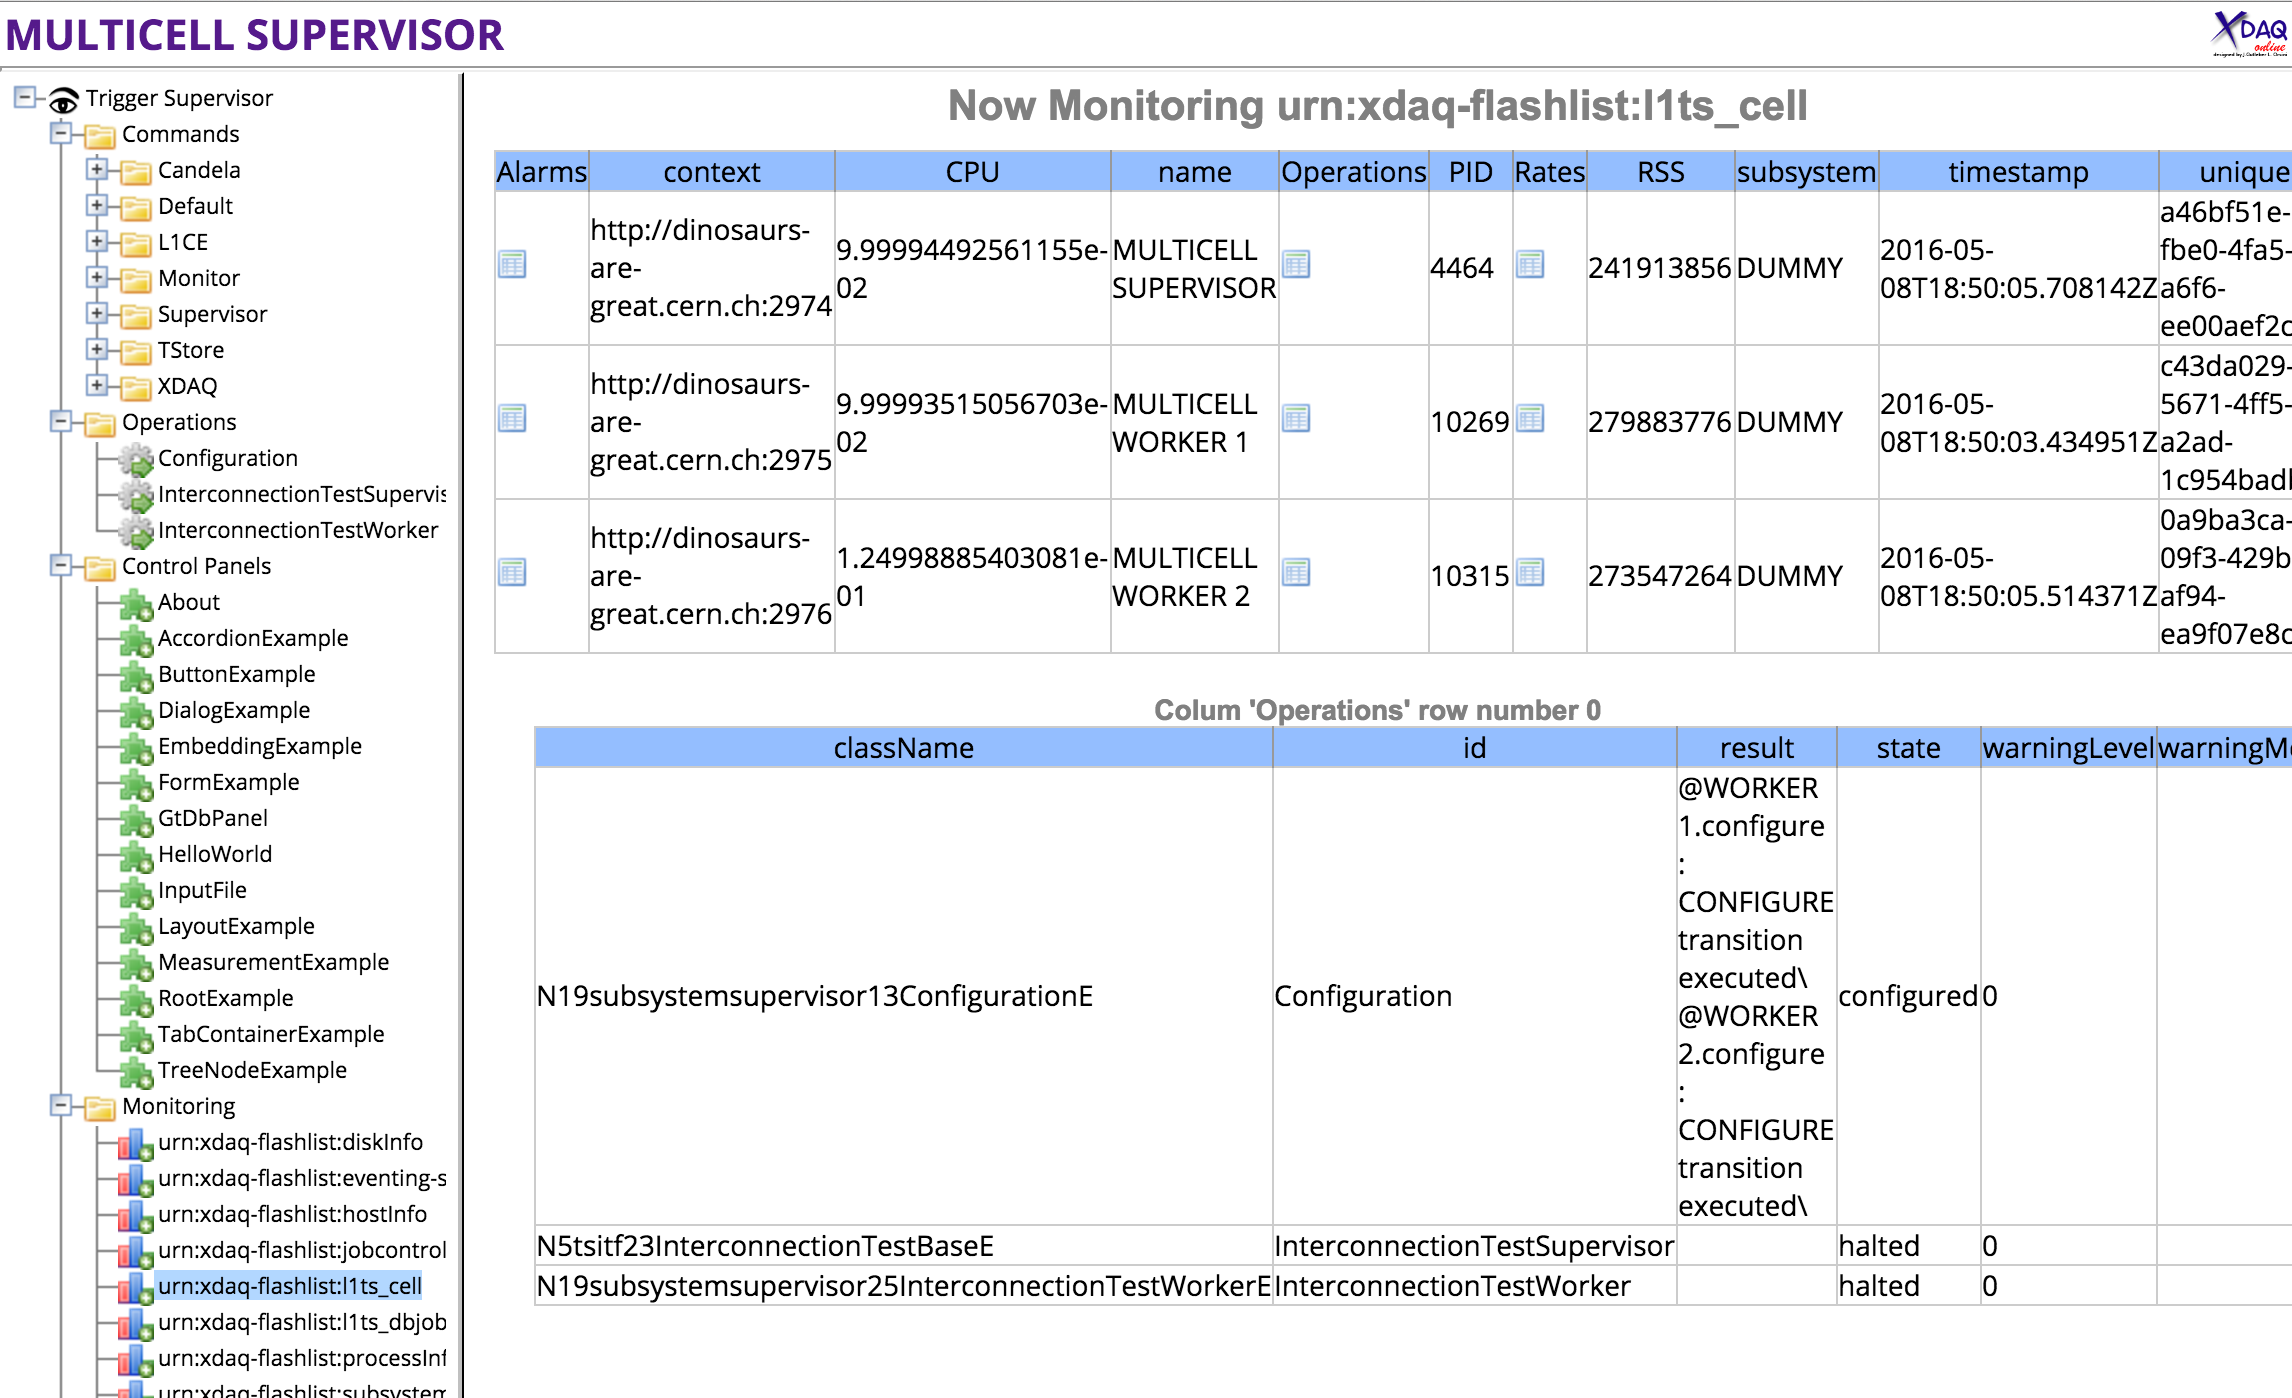
\includegraphics[width=\textwidth]{images/ts2_flashlists}
  \caption{TS 2.x flashlists panel}
  \label{fig:ts2_flashlists}
  \centering
  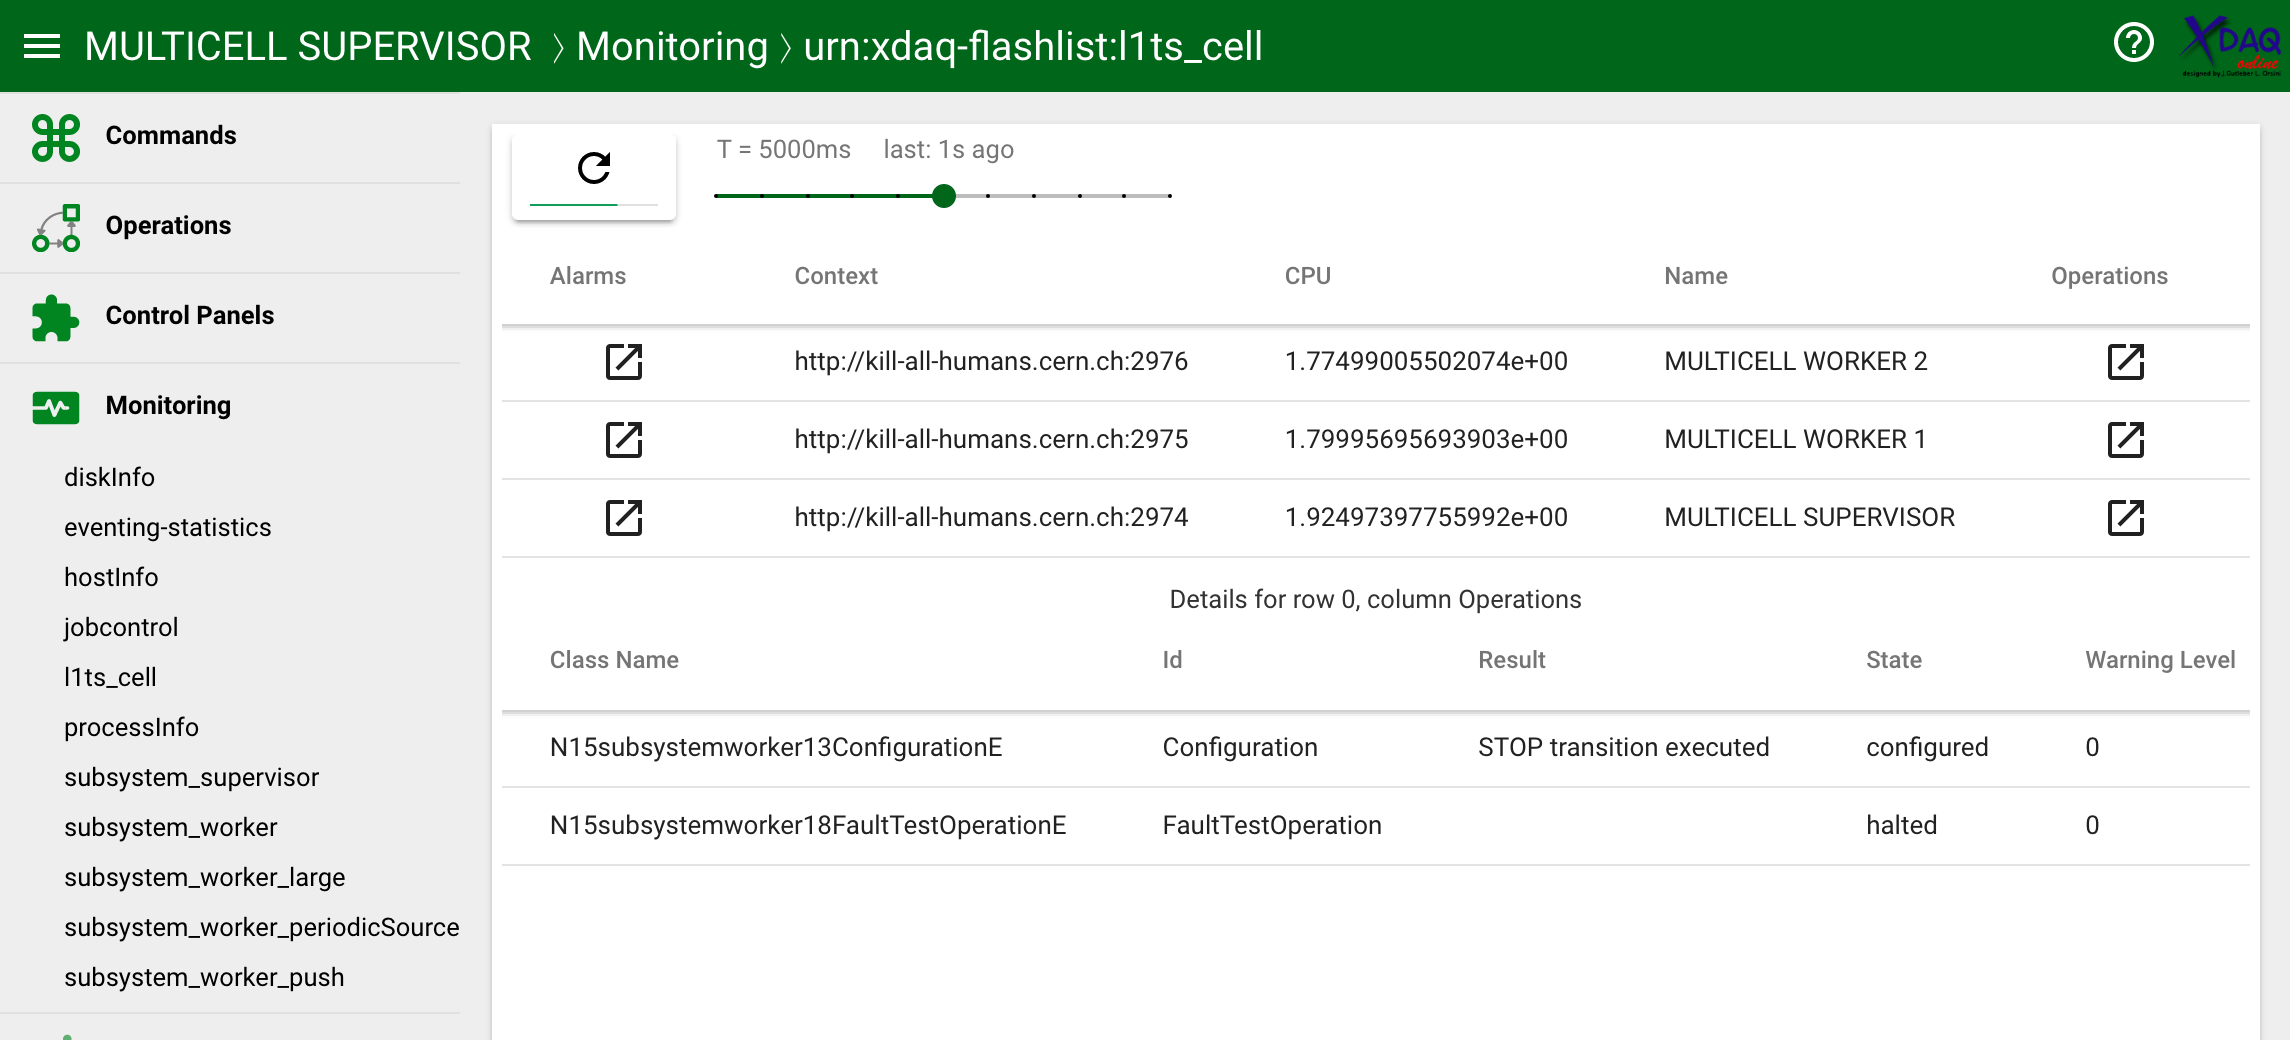
\includegraphics[width=\textwidth]{images/ts3_flashlists}
  \caption{TS 3.x flashlists panel}
  \label{fig:ts3_flashlists}
\end{figure}
% \subsection{Demos}
